\section{Introduction}
\label{sec:introduction}

\begin{figure}
    \centering
    \vspace*{-0.5cm}
    \begin{subfigure}[t]{0.20\textwidth}
        %\hspace*{-0.5cm}
        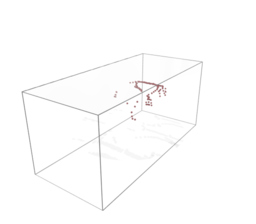
\includegraphics[width=3.75cm,trim={0.5cm 0 1cm 0.75cm},clip]{gfx/overview_small/points/00017}
    \end{subfigure}
    \begin{subfigure}[t]{0.20\textwidth}
        %\hspace*{-0.75cm}
        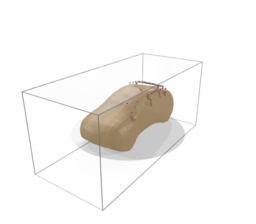
\includegraphics[width=3.75cm,trim={0.5cm 0 1cm 0.75cm},clip]{gfx/overview_small/sdf_points/00017}
    \end{subfigure}\\[-0.1cm]
    \begin{subfigure}[t]{0.5\textwidth}
        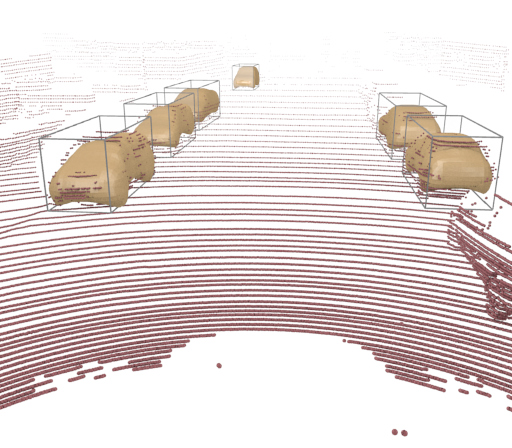
\includegraphics[width=8.25cm,trim={0 8cm 0cm 2cm},clip]{gfx/overview_small/00000}
    \end{subfigure}
    %\vspace*{-4px}
    \caption{{\bf Illustration of the 3D Shape Completion Problem.}
    %On top, we show the Velodyne point cloud of a street scene, annotated with the provided ground truth 3D bounding boxes.
    Top: Given a 3D bounding box and an incomplete point cloud (left, {\color{rred}red}), our goal is to predict the complete shape of the object (right, {\color{rbeige}beige}).
    % missing ground truth shapes.
    %e illustrate an extracted point clouds and the shape completion of our proposed method.
    Bottom: Shape completion results on a street scene from KITTI \cite{Geiger2012CVPR}.
    Learning shape completion on real-world data is challenging due to sparse / noisy observations and missing ground truth.}
    \label{fig:introduction}
    \vspace*{-0.25cm}
\end{figure}

3D shape perception is a long-standing problem both in human \cite{Pizlo2007CAIP,Pizlo2010} and computer vision \cite{Furukawa2013FTCGV}. In both disciplines, a large body of work focuses on 3D reconstruction, \eg, reconstructing objects or scenes from one or multiple views, which is an inherently ill-posed inverse problem where many configurations of shape, color, texture and lighting may result in the very same image \cite{Furukawa2013FTCGV}.
%In human vision, one of the fundamental problems is understanding how the human visual system accomplishes such tasks; in computer vision, in contrast, the goal is to develop 3D reconstruction systems.
Both human and computer vision are related through insights regarding the cues and constraints used by humans to perceive 3D shapes. Motivated by results from human vision \cite{Pizlo2007CAIP,Pizlo2010}, these priors are usually built into 3D reconstruction pipelines through explicit assumptions. Recently, however -- leveraging the success of deep learning -- researchers started to \emph{learn} shape models from data. Predominantly generative models have been used to learn how to generate, manipulate and reason about 3D shapes, \eg, \cite{Girdhar2016ECCV,Brock2016ARXIV,Sharma2016ARXIV,WuNIPS2016,Wu2015CVPR}, thereby offering many interesting possibilities for a wide variety of problems.

\begin{figure*}[t]
    \vspace*{-0.5cm}
	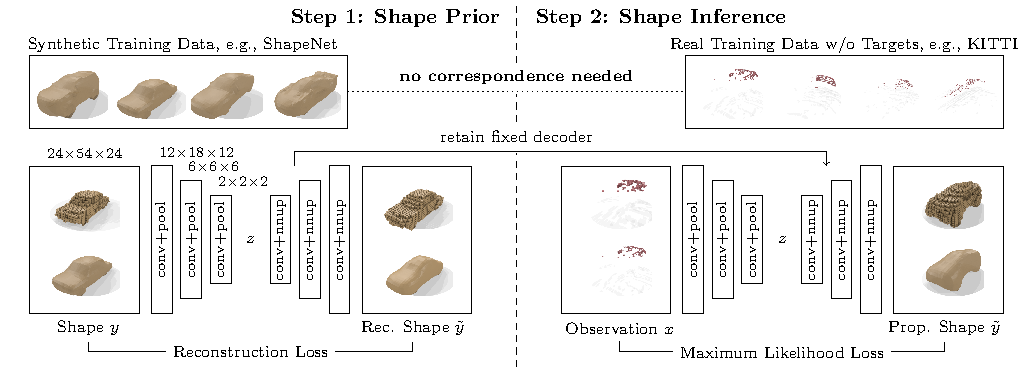
\includegraphics[width=\linewidth]{fig/overview_large}
    %\vspace*{-16px}
	\centering
    \caption{{\bf Proposed Amortized Maximum Likelihood (\AML) Approach to 3D Shape Completion.} We illustrate our amortized maximum likelihood (\AML) approach on KITTI \cite{Geiger2012CVPR}. We consider two steps. In step 1 (left), we use car models from ShapeNet \cite{Chang2015ARXIV} to train a variational auto-encoder (\VAE) \cite{Kingma2013ARXIV}. In our case, the car models are encoded using occupancy grids and signed distance functions (SDFs) at a resolution of $24 \times 54 \times 24$ voxels. In step 2 (right), we retain the pre-trained decoder (with fixed weights) and train a novel deterministic encoder. This network can be trained using a maximum likelihood loss without requiring further supervision. The pre-trained decoder constrains the predictions to valid car shapes while the maximum likelihood loss aligns the predictions with the observations. See text for further details.}
    \label{fig:method}
    \vspace*{-0.25cm}
\end{figure*}
%\documentclass[border=0pt]{standalone}
\usepackage{xcolor}
\usepackage{tikz,tikz-3dplot}
\begin{document}
	\tdplotsetmaincoords{50}{130}
    \begin{tikzpicture}
    % ---------------------------------------------------------
    \node at (5.2, 3.75) {{\bf Step 1: Shape Prior}};
    
    \node[rectangle,draw=black,anchor=west] (prior) at (-1,2.5) {
        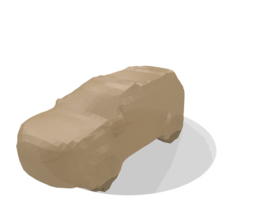
\includegraphics[height=1cm,trim={1cm 1.5cm 3.5cm 3cm},clip]{../gfx/overview_large/00010_target_off}
        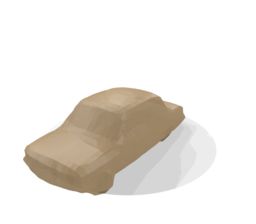
\includegraphics[height=1cm,trim={1cm 1.5cm 3.5cm 3cm},clip]{../gfx/overview_large/00004_target_off}
        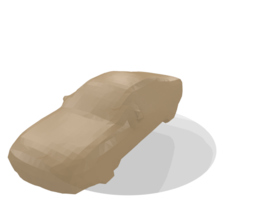
\includegraphics[height=1cm,trim={1cm 1.5cm 3.5cm 3cm},clip]{../gfx/overview_large/00000_target_off}
        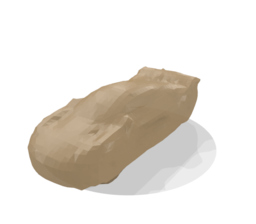
\includegraphics[height=1cm,trim={1cm 1.5cm 3.5cm 3cm},clip]{../gfx/overview_large/00012_target_off}
    };
    \node at (1.6,3.3) {\footnotesize Synthetic Training Data, e.g., ShapeNet};
    
    \node[] (y) at (0, -1.5) {\footnotesize Shape $y$};
    
    \node[rectangle,draw=black,anchor=west] (input) at (-1, 0) {
        \begin{tabular}{c}
            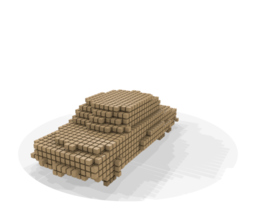
\includegraphics[height=1cm,trim={1cm 1.5cm 3.5cm 3cm},clip]{../gfx/overview_large/00004_target_binvox}\\
            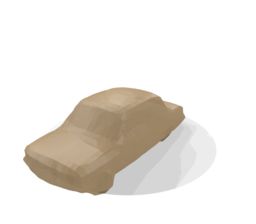
\includegraphics[height=1cm,trim={1cm 1.5cm 3.5cm 3cm},clip]{../gfx/overview_large/00004_target_off}
        \end{tabular}
    };  
    \node at ($(input.north) + (0,0.2)$) {\scriptsize $24{\times}54{\times}24$};
    
    \draw[-] ($(input.north east) + (0.2,0)$) rectangle ($(input.south east) + (0.55,0)$);
    \node[rotate=90] at ($(input.east) + (0.375,0)$) {\scriptsize conv+pool};
    \node[anchor=south west] at ($(input.north east) + (0.2,0)$) {\scriptsize $12{\times}18{\times}12$};
    \draw[-] ($(input.north east) + (0.7,-0.25)$) rectangle ($(input.south east) + (1.05,0.25)$);
    \node[rotate=90] at ($(input.east) + (0.875,0)$) {\scriptsize conv+pool};
    \node[anchor=south west] at ($(input.north east) + (0.7,-0.25)$) {\scriptsize $6{\times}6{\times}6$};
    \draw[-] ($(input.north east) + (1.2,-0.5)$) rectangle ($(input.south east) + (1.55,0.5)$);
    \node[rotate=90] at ($(input.east) + (1.375,0)$) {\scriptsize conv+pool};
    \node[anchor=south west] at ($(input.north east) + (1.2,-0.5)$) {\scriptsize $2{\times}2{\times}2$};
    
    \node (z) at (2.75, 0) {\footnotesize $z$};
    
    \node[rectangle,draw=black,anchor=east] (output) at (6.5, 0) {
        \begin{tabular}{c}
        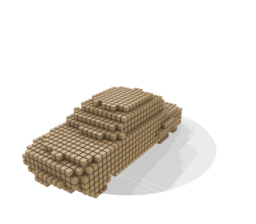
\includegraphics[height=1cm,trim={1cm 1.5cm 3.5cm 3cm},clip]{../gfx/overview_large/00004_prediction_binvox}\\
        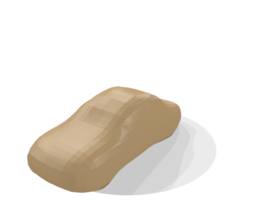
\includegraphics[height=1cm,trim={1cm 1.5cm 3.5cm 3cm},clip]{../gfx/overview_large/00004_prediction_off}
        \end{tabular}
    };
    
    \draw[-] ($(output.north west) - (0.2,0)$) rectangle ($(output.south west) - (0.55,0)$);
    \node[rotate=90] at ($(output.west) - (0.375,0)$) {\scriptsize conv+nnup};
    \draw[-] ($(output.north west) - (0.7,0.25)$) rectangle ($(output.south west) - (1.05,-0.25)$);
    \node[rotate=90] at ($(output.west) - (0.875,0)$) {\scriptsize conv+nnup};
    \draw[-] ($(output.north west) - (1.2,0.5)$) rectangle ($(output.south west) - (1.55,-0.5)$);
    \node[rotate=90] at ($(output.west) - (1.375,0)$) {\scriptsize conv+nnup};
    
    \node (ry) at (5.5, -1.5) {\footnotesize Rec. Shape $\tilde{y}$};
    
    \node[] (L) at (2.75, -1.9) {\footnotesize Reconstruction Loss};
    
    \draw[-] (ry) -- ($(ry) - (0,0.4)$);
    \draw[-] ($(ry) - (0,0.4)$) -- (L);
    \draw[-] (y) -- ($(y) - (0,0.4)$);
    \draw[-] ($(y) - (0,0.4)$) -- (L);
    
    % --
    \draw[-] (3.5, 1.25) -- (3.5, 1.5);
    \draw[-] (3.5, 1.5) -- (12.5, 1.5);
    \draw[->] (12.5, 1.5) -- (12.5, 1.25);
    \node at (7.25, 1.75) {\footnotesize retain fixed decoder};
    \draw[-,dashed] (7.25,-2.15) -- (7.25,1.45);
    \draw[-,dashed] (7.25,2) -- (7.25,2.45);
    \draw[-,dashed] (7.25,3) -- (7.25,4.05);
    
    \node at (7.25, 2.75) {\footnotesize\textbf{no correspondence needed}};
    \begin{scope}[shift={(9,0)}]
    
    % ---------------------------------------------------------
    \node at (0.7, 3.75) {{\bf Step 2: Shape Inference}};
    
    \node[rectangle,draw=black,anchor=east] (inference) at (6.5,2.5) {
        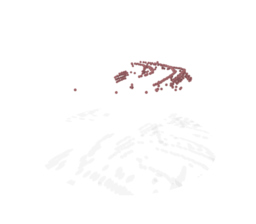
\includegraphics[height=1cm,trim={1cm 1.5cm 3.5cm 3cm},clip]{../gfx/overview_large/00037_input_txt}
        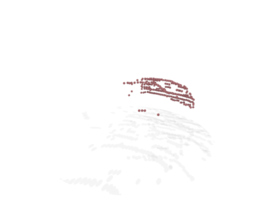
\includegraphics[height=1cm,trim={1cm 1.5cm 3.5cm 3cm},clip]{../gfx/overview_large/00005_input_txt}
        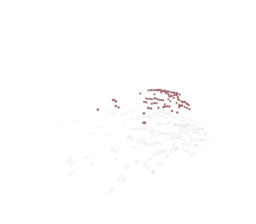
\includegraphics[height=1cm,trim={1cm 1.5cm 3.5cm 3cm},clip]{../gfx/overview_large/00045_input_txt}
        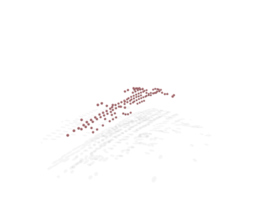
\includegraphics[height=1cm,trim={1cm 1.5cm 3.5cm 3cm},clip]{../gfx/overview_large/00047_input_txt}
    };
    \node at (3.8,3.3) {\footnotesize Real Training Data w/o Targets, e.g., KITTI};
    
    % --
    \draw[-,dotted] (prior) -- (inference);
    
    \node[] (y) at (0, -1.5) {\footnotesize Observation $x$};
    
    \node[rectangle,draw=black,anchor=west] (input) at (-1, 0) {
        \begin{tabular}{c}
        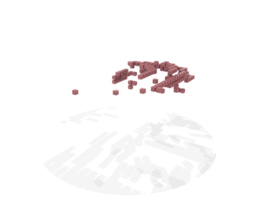
\includegraphics[height=1cm,trim={1cm 1.5cm 3.5cm 3cm},clip]{../gfx/overview_large/00037_input_binvox}\\
        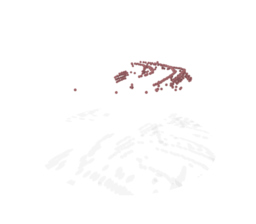
\includegraphics[height=1cm,trim={1cm 1.5cm 3.5cm 3cm},clip]{../gfx/overview_large/00037_input_txt}
        \end{tabular}
    };
    
    \draw[-] ($(input.north east) + (0.2,0)$) rectangle ($(input.south east) + (0.55,0)$);
    \node[rotate=90] at ($(input.east) + (0.375,0)$) {\scriptsize conv+pool};
    \draw[-] ($(input.north east) + (0.7,-0.25)$) rectangle ($(input.south east) + (1.05,0.25)$);
    \node[rotate=90] at ($(input.east) + (0.875,0)$) {\scriptsize conv+pool};
    \draw[-] ($(input.north east) + (1.2,-0.5)$) rectangle ($(input.south east) + (1.55,0.5)$);
    \node[rotate=90] at ($(input.east) + (1.375,0)$) {\scriptsize conv+pool};
    
    \node (z) at (2.75, 0) {\footnotesize $z$};
    
    \node[rectangle,draw=black,anchor=east] (output) at (6.5, 0) {
        \begin{tabular}{c}
        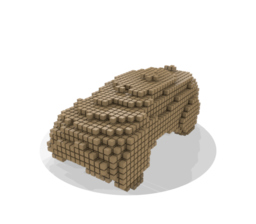
\includegraphics[height=1cm,trim={1cm 1.5cm 3.5cm 3cm},clip]{../gfx/overview_large/00037_prediction_binvox}\\
        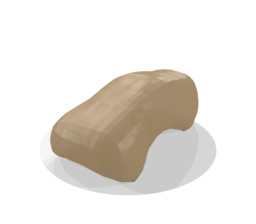
\includegraphics[height=1cm,trim={1cm 1.5cm 3.5cm 3cm},clip]{../gfx/overview_large/00037_prediction_off}
        \end{tabular}
    };
    
    \draw[-] ($(output.north west) - (0.2,0)$) rectangle ($(output.south west) - (0.55,0)$);
    \node[rotate=90] at ($(output.west) - (0.375,0)$) {\scriptsize conv+nnup};
    \draw[-] ($(output.north west) - (0.7,0.25)$) rectangle ($(output.south west) - (1.05,-0.25)$);
    \node[rotate=90] at ($(output.west) - (0.875,0)$) {\scriptsize conv+nnup};
    \draw[-] ($(output.north west) - (1.2,0.5)$) rectangle ($(output.south west) - (1.55,-0.5)$);
    \node[rotate=90] at ($(output.west) - (1.375,0)$) {\scriptsize conv+nnup};
    
    \node (ry) at (5.5, -1.5) {\footnotesize Prop. Shape $\tilde{y}$};
    
    \node[] (L) at (2.75, -1.9) {\footnotesize Maximum Likelihood Loss};
    
    \draw[-] (ry) -- ($(ry) - (0,0.4)$);
    \draw[-] ($(ry) - (0,0.4)$) -- (L);
    \draw[-] (y) -- ($(y) - (0,0.4)$);
    \draw[-] ($(y) - (0,0.4)$) -- (L);
    \end{scope}
    \end{tikzpicture}
\end{document}


In this paper, we focus on the problem of inferring and completing 3D shapes based on sparse and noisy 3D point observations as illustrated in \figref{fig:introduction}.
%This problem has many relevant applications, including 
This problem occurs when only a single view of an individual object is provided or large parts of the object are occluded as, \eg, in autonomous driving applications.
%The problem is, however, also closely related to surface reconstruction \cite{Berger2014EUROGRAPHICS} and, thus, has relevant applications in computer graphics, as well.
Existing approaches to shape completion can be roughly categorized into data-driven and learning-based methods. The former usually rely on learned shape priors and formulate shape completion as optimization problem over the corresponding (lower-dimensional) latent space \cite{Engelmann2016GCPR,Bao2013CVPR,Dame2013CVPR,Guney2015CVPR}. These approaches have demonstrated impressive performance on real data, \eg, on KITTI \cite{Geiger2012CVPR}.
% as demonstrated in \cite{Engelmann2016GCPR}.
Learning-based approaches, in contrast, assume a fully supervised setting in order to directly learn shape completion on synthetic data \cite{Riegler2017THREEDV,SmithARXIV2017,Dai2017CVPRa,Sharma2016ARXIV,Fan2016ARXIV,Rezende2016ARXIV}. As full supervision is required, the applicability of these approaches to real data is limited.
% and has -- to the best of our knowledge -- not been addressed.
However, learning-based approaches offer advantages in terms of efficiency: a forward pass of the learned network is usually sufficient. In practice, both problems -- the optimization problem of data-driven approaches and the required supervision of learning-based approaches -- limit the applicability of state-of-the-art shape completion methods to real data.

%In this work, we propose a model which tackles this problem.
%address both problems: the need of annotated training data and the drawbacks of computationally involved optimization problems.
%In particular, we utilize ShapeNet \cite{Chang2015ARXIV} to learn a strong shape prior using variational auto-encoders \cite{Kingma2013ARXIV}.

% ag: add something of this again?
%We hypothesize that using a strong prior of possible shapes allows us to learn shape completion under weak supervision, \ie, only given knowledge about the object category at hand. On real data, we additionally assume knowledge about the object location in the form of bounding boxes which can be provided by an object detector.
%
%By learning shape completion using deep networks, we additionally reduce the problem to a forward pass of the trained network. 
%{\color{red} Question: can I stop citing a paper after I first cited it (except for related work)?}
% ag: yes.
%\textbf{Contribution.}
%
To tackle these problems, this work proposes an amortized maximum likelihood approach for 3D shape completion.
More specifically, we first learn a shape model on synthetic data using a variational auto-encoder \cite{Kingma2013ARXIV} (\cf Figure \ref{fig:method}, step 1). Shape completion can then be formulated as maximum likelihood problem -- in the spirit of \cite{Engelmann2016GCPR}.
Instead of maximizing the likelihood independently for distinct observations, however, we follow the idea of amortized inference \cite{Gersham2014COGSCI} and \emph{learn} to predict the maximum likelihood solutions directly given the observations.
Towards this goal, we train a new encoder which embeds the observations in the same latent space using an unsupervised maximum likelihood loss (\cf Figure \ref{fig:method}, step 2). This allows us to learn 3D shape completion in challenging real-world situations, \eg, on KITTI.
Using signed distance functions to represent shapes, we are able to obtain sub-voxel accuracy while applying regular 3D convolutional neural networks to voxel grids of limited resolution, yielding a highly efficient inference method.
For experimental evaluation, we introduce two novel, synthetic shape completion benchmarks based on ShapeNet and ModelNet. On KITTI, we further compare our approach to the work of Engelmann \etal \cite{Engelmann2016GCPR} -- the only related work which addresses shape completion on KITTI.
Our experiments demonstrate that we obtain shape reconstructions which rival data-driven techniques while significantly reducing inference time.
Our code and datasets are made publicly available\footnote{\url{https://avg.is.tuebingen.mpg.de/research_projects/3d-shape-completion}.}.
%The presented experiments support our claim that shape completion can be learned  shape priors allow weakly-supervised learning of shape completion.

This paper is structured as follows: we discuss related work in Section \ref{sec:related-work}. In Section \ref{sec:method} we describe our amortized maximum likelihood framework for weakly-supervised shape completion. We present experimental results in Section \ref{sec:experiments} and conclude in Section \ref{sec:conclusion}.
